\documentclass[a4paper]{article} 
\addtolength{\hoffset}{-2.25cm}
\addtolength{\textwidth}{4.5cm}
\addtolength{\voffset}{-3.25cm}
\addtolength{\textheight}{5cm}
\setlength{\parskip}{0pt}
\setlength{\parindent}{0in}

%----------------------------------------------------------------------------------------
%	PACKAGES AND OTHER DOCUMENT CONFIGURATIONS
%----------------------------------------------------------------------------------------

\usepackage{blindtext} % Package to generate dummy text
\usepackage{charter} % Use the Charter font
\usepackage[utf8]{inputenc} % Use UTF-8 encoding
\usepackage{microtype} % Slightly tweak font spacing for aesthetics
\usepackage[english, ngerman]{babel} % Language hyphenation and typographical rules
\usepackage{amsthm, amsmath, amssymb} % Mathematical typesetting
\usepackage{float} % Improved interface for floating objects
\usepackage[final, colorlinks = true, 
            linkcolor = black, 
            citecolor = black]{hyperref} % For hyperlinks in the PDF
\usepackage{graphicx, multicol} % Enhanced support for graphics
\usepackage{xcolor} % Driver-independent color extensions
\usepackage{marvosym, wasysym} % More symbols
\usepackage{rotating} % Rotation tools
\usepackage{censor} % Facilities for controlling restricted text
\usepackage{listings, style/lstlisting} % Environment for non-formatted code, !uses style file!
\usepackage{pseudocode} % Environment for specifying algorithms in a natural way
\usepackage{style/avm} % Environment for f-structures, !uses style file!
\usepackage{booktabs} % Enhances quality of tables
\usepackage{tikz-qtree} % Easy tree drawing tool
\tikzset{every tree node/.style={align=center,anchor=north},
         level distance=2cm} % Configuration for q-trees
\usepackage{style/btree} % Configuration for b-trees and b+-trees, !uses style file!
\usepackage[backend=biber,style=numeric,
            sorting=nyt]{biblatex} % Complete reimplementation of bibliographic facilities
\addbibresource{ecl.bib}
\usepackage{csquotes} % Context sensitive quotation facilities
\usepackage[yyyymmdd]{datetime} % Uses YEAR-MONTH-DAY format for dates
\renewcommand{\dateseparator}{-} % Sets dateseparator to '-'
\usepackage{fancyhdr} % Headers and footers
\pagestyle{fancy} % All pages have headers and footers
\fancyhead{}\renewcommand{\headrulewidth}{0pt} % Blank out the default header
\fancyfoot[L]{} % Custom footer text
\fancyfoot[C]{} % Custom footer text
\fancyfoot[R]{\thepage} % Custom footer text
\newcommand{\note}[1]{\marginpar{\scriptsize \textcolor{red}{#1}}} % Enables comments in red on margin

%----------------------------------------------------------------------------------------

\usepackage{multirow}
\usepackage{graphicx}
\usepackage[figurename=Fig.]{caption}
\begin{document}

%-------------------------------
%	TITLE SECTION
%-------------------------------

\fancyhead[C]{}
\hrule \medskip % Upper rule
\begin{minipage}{0.295\textwidth} 
\raggedright
\footnotesize

\end{minipage}
\begin{minipage}{0.4\textwidth} 
\centering 
\large 
EE 556 Project\\ 
\normalsize 
\end{minipage}
\begin{minipage}{0.295\textwidth} 
\raggedleft
\today\hfill\\
\end{minipage}
\medskip\hrule 
\bigskip

%-------------------------------
%	CONTENTS
%-------------------------------

\section{Code}
In this project, I implement the ZOO attacks in Matlab to evade a DNN model trained on the MNIST dataset(source code: \href{https://github.com/Moirai7/ee556/}{Github}).

The key idea of the ZOO attacks is to estimate the gradient of a black-box model. The approximate gradient is computed with the zeroth-order optimazation method instead of using the actual backpropagation on the targeted model. 

First, for a targeted attack, the loss function is 
\begin{equation}
f(x,t) = max\{max_{i\neq t}log[F(x)]_i - log[F(x)]_t, 0\}
\end{equation} 
Minimizing the loss function requires to attains the highest confidence score for the targeted class $t$.

Then, ZOO attacks use the symmetric difference quotient to estimate the gradient on the loss function.
\begin{equation}
g_i = \frac{\partial f(x)}{\partial x_i} = \frac{f(x+he_i)-f(x-he_i)}{2h}
\end{equation}

To reduce the computational complexity, I implemented two algorithms ZOO-ADAM and ZOO-Newton proposed by \cite{1}. Both of them first randomly pick a batch of coordinates. Then ZOO-ADAM method calculates the first-order of the loss function to compute the best coordinate update. Meanwhile, the ZOO-Newton method calculates the gradient and Hessian for $x_i$ to update the coordinate.


\section{Result}


\subsection{Attack Rates}
It takes a long time to calculate the adversarial samples on the whole test dataset(about one day for 300 adversarial samples on my computer). To evaluate the performance of the attack methods, I first selected 1000 images that could be correctly classified as their true labels and randomly select a target label. \textbf{The success attack rate of both algorithms are 100\%.}

Then I evaluated the attack rate for different target labels.
I selected 200 images and generated 9 adversarial samples for each image with target classes that are different from their true labels. Table \ref{ar} shows the attack success rate with those two attack methods. Both of them can reach a 100\% attack rate with all target classes. 

\begin{table}[h]
\centering
\begin{tabular}{ccc}
\hline
Target Label&ZOO-ADAM&ZOO-Newton\\
\hline
0& 100\%&100\%\\
1& 100\%&100\%\\
2& 100\%&100\%\\
3& 100\%&100\%\\
4& 100\%&100\%\\
5& 100\%&100\%\\
6& 100\%&100\%\\
7& 100\%&100\%\\
8& 100\%&100\%\\
9& 100\%&100\%\\
\hline
\end{tabular}
\label{ar}
\caption{Attack Rate}
\end{table}
In practice, the ZOO-ADAM method is faster than the ZOO-Newton method.
\textbf{For ZOO-ADAM attack the average number of classifier queries to achieve a successful attack is 883.8.
For the ZOO-Newton attack, the average number of queries is 1471.1. }Each query randomly selects 128 coordinates to update.


As shown in Fig.1, the human can see there are some noises on the adversarial samples but we still can identify true labels for those generated samples. \textbf{Generally, the adversarial samples are imperceptible.}
\begin{figure}
\centering
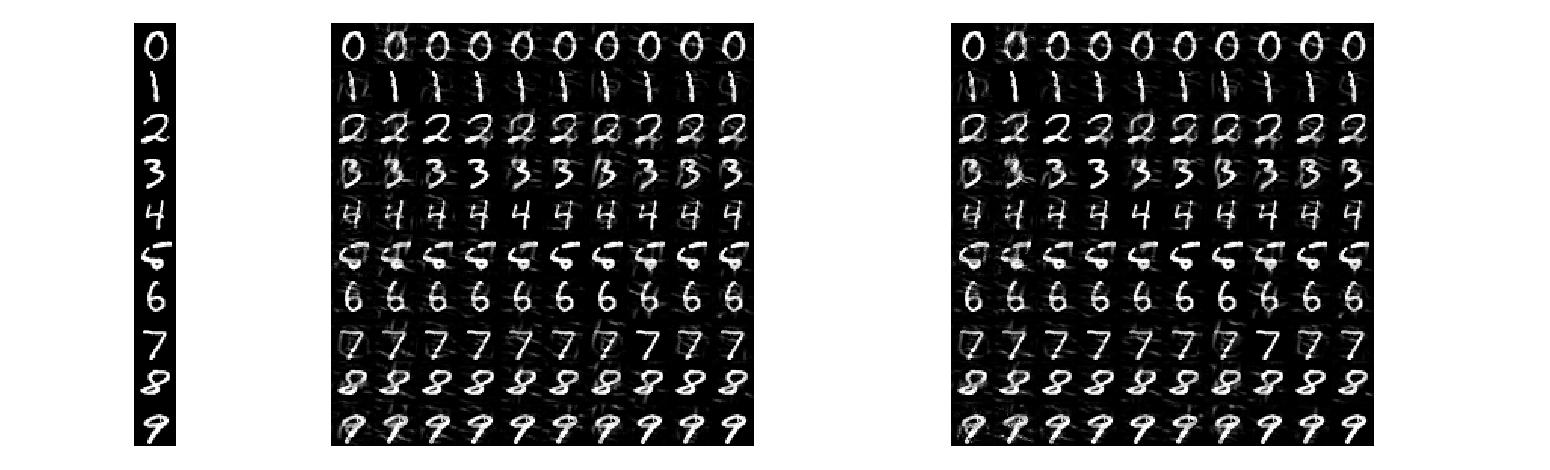
\includegraphics[scale=0.3]{resjpg.jpg}
\label{ae}
\caption{Successful adversarial examples in MNIST. Each row displays adversarial examples from the sampled images. Each column indexes the targeted class(0-9) for attack.}
\end{figure}

\subsection{Defense}
One way to defend against this attack is to train another model to differentiate the adversarial samples.
I trained neural networks using the same architecture as the classification model. 70\% generated adversarial examples and their corresponding original images are used for training and others are used to test the defense model. 
Fig.2 and Fig.3 are the performance of the defense model. \textbf{The AUC of the defense model for the ZOO-ADAM attack on the test dataset is 95.36\%. For the ZOO-Newton attack, it is 94.74\%}.

\begin{figure}
\centering
\begin{minipage}[t]{0.45\textwidth}
\centering
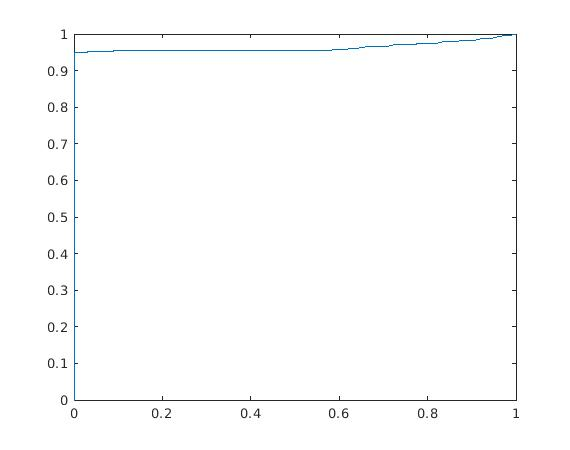
\includegraphics[scale=0.3]{roc.jpg}
\label{roc}
\caption{Performance of the defense method for the ZOO-ADAM attack(neural networks)}
\end{minipage}
\begin{minipage}[t]{0.45\textwidth}
\centering
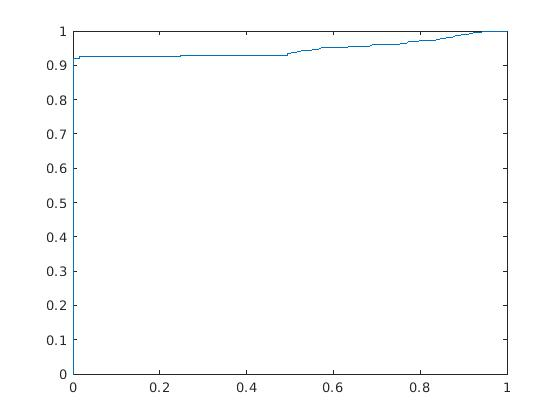
\includegraphics[scale=0.3]{roc_newton.jpg}
\label{roc}
\caption{Performance of the defense method for the ZOO-Newton attack(neural networks)}
\end{minipage}
\end{figure}

For the MNIST dataset, I found the generate samples have an obvious characteristic. There are more pixels with the gray color in adversarial samples. Fig. 4  is the frequency of 256 different intensities on 200 original samples and 200 adversarial samples. If we filter out the white(256) and black(0), the differences between the generated samples and the original samples are more significant as shown in Fig. 5.

\begin{figure}
\centering
\begin{minipage}[t]{0.45\textwidth}
\centering
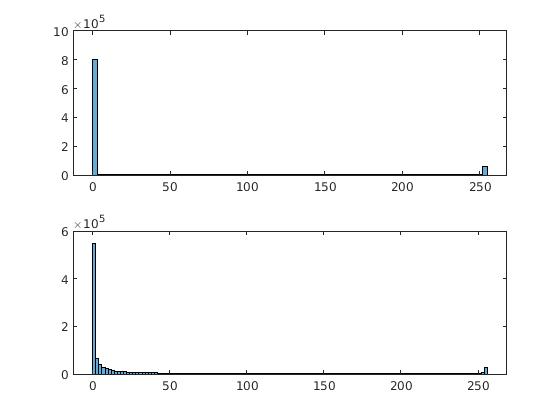
\includegraphics[scale=0.3]{freq2.jpg}
\label{freq2}
\caption{The frequency of different intensities (from 0 to 255)}

\end{minipage}
\begin{minipage}[t]{0.45\textwidth}
\centering
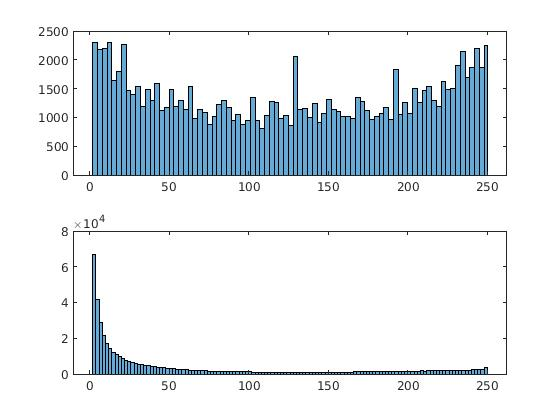
\includegraphics[scale=0.3]{freq.jpg}
\label{freq}
\caption{The frequency of different intensities (from 2 to 250)}
\end{minipage}
\end{figure}

So we could calculate the ratio of ``gray color" (intensities from 2 to 90) in one unknown image to detect the attack.
First, we use 70\% generated adversarial examples and their corresponding original images to define the threshold that would be classified as attacks. Fig. 6 is the ratio of gray color in original images and adversarial images. Based on the statical analysis, we simply define the following decision rules: if the ratio is more than 9\%, we can classify the images as attacks with 100\%; if the ratio is more than 6\% and less than 9\%, the probability the image is not an adversarial example is 70\%; if it is more than 2\% and less than 6\%, the probability the image is not an adversarial example is 90\%; otherwise, the probability the image is not an adversarial example is 70\%.

Then we use these simple rules to calculate the AUC on the test dataset. Fig. 7 and Fig.8 are the performance of this defense method.
And \textbf{the AUC for the ZOO-ADAM attack is 97.66\%; for the ZOO-Newton attack it is 98.36\%}.
\begin{figure}
\centering
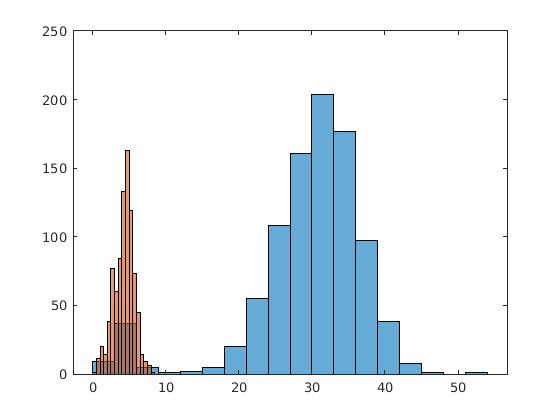
\includegraphics[scale=0.5]{freq3.jpg}
\label{freq3}
\caption{The ratio of gray color in original images and adversarial images}
\end{figure}

\begin{figure}
\centering
\begin{minipage}[t]{0.45\textwidth}
\centering
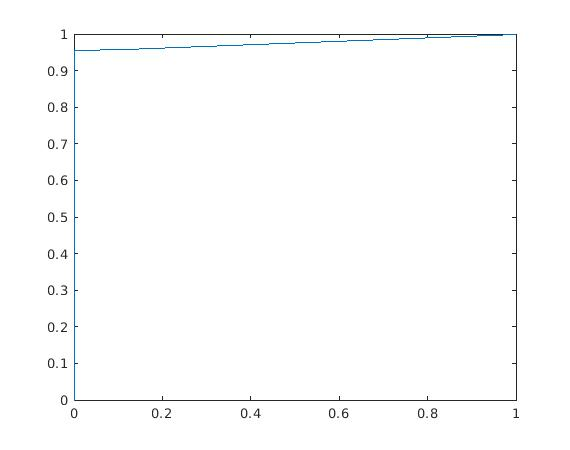
\includegraphics[scale=0.3]{roc2.jpg}
\label{roc2}
\caption{Performance of the defense method for the ZOO-ADAM attack(gray color)}
\end{minipage}
\begin{minipage}[t]{0.45\textwidth}
\centering
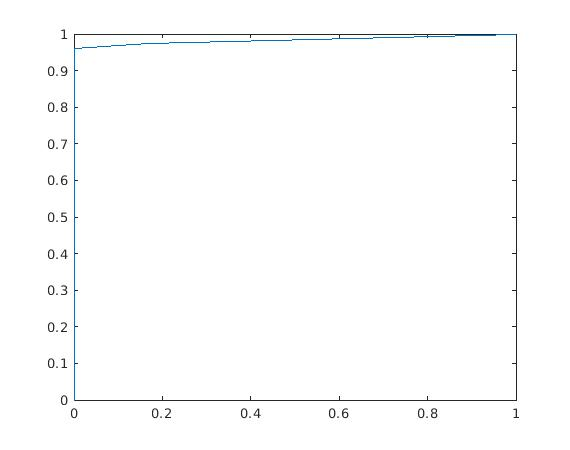
\includegraphics[scale=0.3]{roc2_newton.jpg}
\label{roc2}
\caption{Performance of the defense method for the ZOO-Newton attack(gray color)}
\end{minipage}
\end{figure}

\begin{thebibliography}{9}
\bibitem{1}
Chen, P. Y., Zhang, H., Sharma, Y., Yi, J., \& Hsieh, C. J. (2017). ZOO: Zeroth order optimization based black-box attacks to deep neural networks without training substitute models. ArXiv.
\end{thebibliography}

\end{document}
